\subsubsection{Incremento 5}
\textit{\textbf{Periodo}: dal 2021-03-09 al 2021-03-12}

\myparagraph{Obiettivi}
Gli obiettivi definiti per questo incremento sono i seguenti:
\begin{itemize}
\item incremento della documentazione;
\item preparazione alla progettazione in dettaglio e codifica del prodotto;
\item approfondimento personale per requisiti non sviluppati dal Proof of Concept\ped{G}.
\end{itemize}

\myparagraph{Attività}
Per raggiungere gli obiettivi, vengono svolte le seguenti attività:
\begin{itemize}

\item \textbf{configurazione prodotto}:
\begin{itemize}
\item creazione nuove repository\ped{G} e ambienti di sviluppo;
\item configurazione del prodotto come fatto per Proof of Concept\ped{G}, con opportune correzioni basate sulle segnalazioni del colloquio con proponente e in sede di Technology baseline\ped{G}.
\end{itemize}

\item \textbf{approfondimento tecnologie}:
\begin{itemize}
\item ricerca best practices per le tecnologie da utilizzare;
\item studio di tecnologie mancanti nel Proof of Concept\ped{G}.
\end{itemize}

\item \textbf{ampliamento documentazione e verifiche}:
\begin{itemize}
\item aggiornamento \PdPv{2.0.0} per pianificazione dei successivi incrementi;
\item incremento del \Glossariov{2.0.0};
\item rilevazione e registrazione di metriche, esiti di verifica e obiettivi di qualità;
\item aggiornamento dei rischi rilevati;
\item calcolo e registrazione del consuntivo di periodo.
\end{itemize}

\end{itemize}
\myparagraph{Diagramma di Gantt}

\begin{figure}[H]
\centering

\centerline{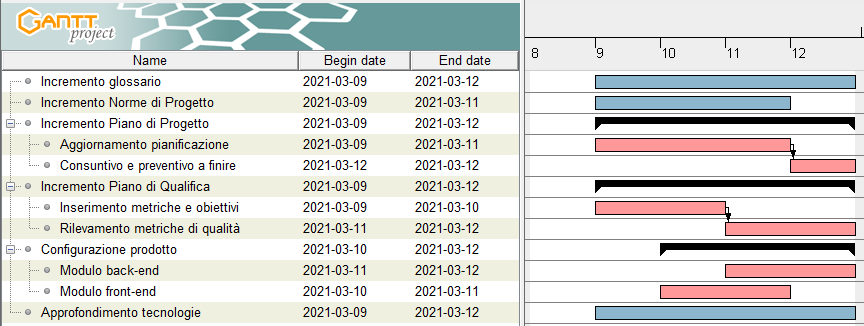
\includegraphics[scale=0.6]{res/Pianificazione/Fasi/CodificaIncrementi/ganttIncremento5}}
\caption{Diagramma di Gantt per l'incremento 5}
\end{figure}

